\documentclass[sigconf]{acmart}

\input{format/final}

\begin{document}
\title{Recipe Ingredient Analysis}


\author{Sushant Athaley}
\affiliation{%
  \institution{Indiana University}
}
\email{sathaley@iu.edu}

% The default list of authors is too long for headers}
\renewcommand{\shortauthors}{G. v. Laszewski}


\begin{abstract}
Food is the unavoidable part of day to day of human life. Ingredients play a major role or are the basic requirement in preparation of any kind of food. We can find the humongous list of ingredients getting used across globally along with other details which constitutes to big data. We explore ingredients getting used in various recipes across the globe to understand most used ingredient, key ingredients of various cuisine and the relationship between the ingredients to find out closely related ingredients which can always provide great dish if used together.
\end{abstract}

\keywords{i523, hid302, big data, ingredient, recipe, analysis, python, gephi}

\maketitle

\section{Introduction}
TBD
The emergence of big data challenges also gave rise to the various technologies which can be used to solve big data problem. Typically to solve big data, we need to consider two types of technologies, data capture and storage, and data analysis. We evaluate capabilities of two popular technologies Hadoop and MongoDB to understand their features and power to solve big data problem. We get started with the section \emph{Big Data} which captures big data definition and characteristics. Section \emph{Conclusion} concludes the study. 

Main focus of this study is on the ingredients used in various recipes across the cuisines. We have collected recipe ingredient data set from Kaggle \cite{www-kaggle} to analyze most used ingredients and ingredient relationship.

\section{Ingredient}
Food is defined as ``Edible or potable substance (usually of animal or plant origin), consisting of nourishing and nutritive components such as carbohydrates, fats, proteins, essential mineral and vitamins, which (when ingested and assimilated through digestion) sustains life, generates energy, and provides growth, maintenance, and health of the body'' \cite{www-businessdictionary}. Thus food is the basic necessity for human for the sustainability. Food can be eaten row, cooked or processed. As human race evolved over period of time, the way we eat food is also evolved. Food cooking is just not the basic necessity but its the art and science in today's era. Food preparation consists of various cooking techniques, tools and ingredients to make it palatable or edible by humans. Ingredient is by far the most important part of any food or recipe preparation. Recipe consists of list of ingredients and the set of instruction to cook particular food dish \cite{www-collinsdictionary}. Ingredient is defined as ``Any of the foods or substances that are combined to make a particular dish'' \cite{www-oxforddictionaries}. Ingredients impart various flavours, aroma, texture and color to the cooking dish. Ingredients are mostly derived from vegetables, fruits, nuts, grains, living organisms, herbs, flowers and spices. It comes in both solid and liquid forms. Another characteristic of ingredients is the nutritional value they provides which is essential for the human body.

\section{Ingredient Analytics}
Ingredients characteristics and combination of other related data provides opportunity to analyze ingredient in different ways. Analysis of the flavors present in ingredient can provide us with the categorization of different ingredient by the flavour profile which can be helpful in deciding substitute ingredient if certain ingredient is not present or pairing ingredient from different flavour categories to construct the dish as per the taste required. 

TBD

\section{Project}
This project study is conducted to analyze ingredients getting used in various recipes across the cuisines to find out
\begin{itemize}
\item Most used ingredients across cuisines or globally
\item Key ingredients used by cuisines
\item Ingredient relationship or connection to understand the related ingredients
\end{itemize}

\subsection{Technologies}
Technologies and tools used in this projects are
\begin{itemize}
\item Python version 3.6 is used for data load and processing
\item Gephi 0.9.2 for visualization
\item Spyder 3.0 as a Python IDE
\end{itemize}

\subsection{Methodology}
First step was to source the data. We were interested in data set which provides recipe information along with the ingredient used in the recipe. Since we wanted to analyze distribution across cuisine, data should also contain cuisine tagging. This data set can be generated by pulling recipe data from various online applications or pick from publicly available data-sets. We finalized publicly available data-set at Kaggle application satisfying need for this project.

Figure \ref{f:methodology} shows methodology used for this project to analyze ingredient data.
\begin{figure}[!ht]
  \centering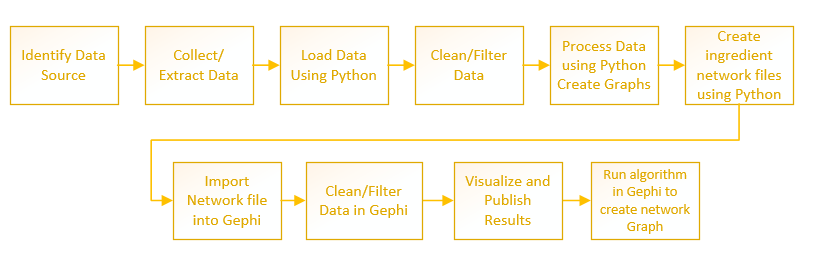
\includegraphics[width=\columnwidth]{images/methodology.PNG}
  \caption{Flowchart of the Methodology to Analyze Ingredients }\label{f:methodology}
\end{figure}

DataSet is loaded through Python script and further processed to clean the data. This cleaned data then processed to analyze ingredient distribution across cuisine and per cuisine. Gephi software is used to analyze the relationship and to find out the ingredient modularity. Python script is used to create the required network files required by the Gephi tool. Gephi requires Nodes and relationship in terms of Edges between the nodes for the analysis. Python script is used to create Node and Edges file in excel format so that it can be imported in Gephi. Distinct ingredients used across recipe becomes the nodes. Edges or relationship between ingredients are derived by relating ingredients appearing in same recipe. All ingredient in same recipe are related to each other.
Network files created by Python are imported in Gephi to produce graph for the visualization. Gephi tools data laboratory is used to clean up the data and filters to provide nice network visualization. 

\subsection{Data Set}
DataSet for this study is sourced from Kaggle application \cite{www-kaggle}. This dataset is publicly available and featured in ``What's Cooking?'' competition. This dataset is in JSON format and of 12MB size. This data set contains recipe id, cuisine and list of ingredients as described in Figure \ref{c:data-structure}.
\begin{figure}[htb]
\begin{verbatim}
{
 "id": 24717,
 "cuisine": "indian",
 "ingredients": [
     "tumeric",
     "vegetable stock",
     "tomatoes",
     "garam masala",
     "naan",
     "red lentils",
     "red chili peppers",
     "onions",
     "spinach",
     "sweet potatoes"
 ]
 },
\end{verbatim}
\caption{Ingredient Data Structure}\label{c:data-structure}
\end{figure}
This dataset contains total 39774 recipes across various cuisines. We used two different methods to load this data. Cuisine and ingredient analysis is done by loading data into \emph{pandas dataframe} and to analyze ingredient relationship data has been loaded into \emph{json} object. Figure \ref{c:data-loading} shows code for data loading used in this project.
\begin{figure}[htb]
\begin{verbatim}
#read the ingredient data using pandas
dfTrain = pd.read_json('./data/train.json')


#load data using json
dataFilePath="./data/train.json"
with open(dataFilePath) as data_file:    
    data = json.load(data_file)
\end{verbatim}
\caption{Data Loading}\label{c:data-loading}
\end{figure}

Ingredient extraction from the data structure and processing was challenging as ingredients are listed comma separated for each recipe. Also ingredient list can vary by recipe and there is no proper structure. Another issue with the ingredient list is ingredient appears in various forms but it's the same ingredient which gives duplicate data. For example salt appears as salt, kosher salt, Morton Salt, sea salt, table salt, Himalayan salt, fine sea salt, low sodium salt, fine salt. This is same ingredient but come across in recipe as different ingredient and getting counted as separate ingredient in the analysis. Some ingredients are listed along with measures like (10 oz.) frozen chopped spinach, (10 oz.) frozen chopped spinach, thawed and squeezed dry, (14.5 oz.) diced tomatoes and getting counted as separate ingredient. Some ingredients are listed along with the brand name like KRAFT Reduced Fat Shredded Mozzarella Cheese, Johnsonville Smoked Sausage, Johnsonville Mild Italian Sausage Links etc and also constitutes to the ingredient list. This variation makes difficult to get the proper ingredient list for the analysis. Extensive work is needed to clean and correct the noisy data so that proper analysis can be carried out. This correction process is not carried out as part of this project.

Certain ingredients like salt or water etc should be avoided from the analysis as those are not the ingredient we are looking for the analysis. We tried to clean such elements during ingredient relationship analysis but we had little success as those ingredients are present in database in various forms.  

\subsection{Analysis and Findings}

\subsubsection{Recipe Distribution By Cuisine}
We first analyze entire dataset to understand the total number of recipes and their distribution across various cuisines. We use Pythons Panda library to get the total recipe count as 39774 and plot the distribution. Figure \ref{f:Number_of_recipes_by_cuisine} shows number of recipes per cuisine. Dataset is heavily dominated by Italian cuisine followed by Mexican cuisine and with very less recipes from Russian and Brazilian cuisines. This also highlights another shortcoming of the dataset that it doesn't have equal representation of all cuisines which might give us biased analysis.
\begin{figure}[!ht]
  \centering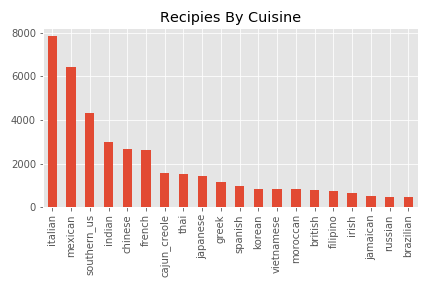
\includegraphics[width=\columnwidth]{images/Number_of_recipes_by_cuisine.png}
  \caption{Recipe Distribution By Cuisine }\label{f:Number_of_recipes_by_cuisine}
\end{figure}

\subsubsection{Most Used Ingredients All Cuisines}
Second analysis is carried out to understand top 20 ingredients getting used across cuisine or globally. Ingredient \emph{Salt} is obvious topper followed by \emph{Oil} and \emph{Onions}. This also proves our craving for saltiness and fat. Figure \ref{f:Ingredient_Distribution} shows top 20 ingredient across cuisines. 
\begin{figure}[!ht]
  \centering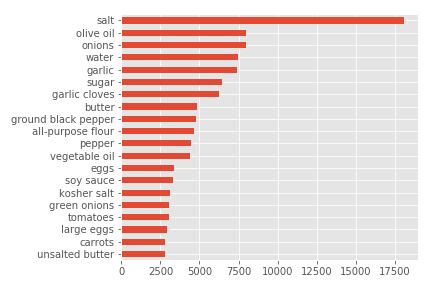
\includegraphics[width=\columnwidth]{images/Ingredient_Distribution.png}
  \caption{Top 20 Ingredients }\label{f:Ingredient_Distribution}
\end{figure}

\subsubsection{Ingredients Distribution By Cuisines}
Third analysis is carried out to understand key ingredient for each cuisine. This key ingredients defines those cuisines and provide unique test characterized by that cuisine. We limited ingredient list to top 10 to get the key ingredients for each cuisine. Figure \ref{f:italian_10_most_used_ingredients} shows top 10 key ingredient used in the Italian cuisines. 
\begin{figure}[!ht]
  \centering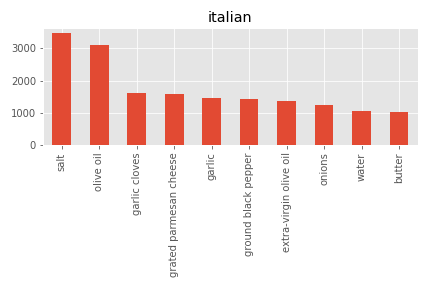
\includegraphics[width=\columnwidth]{images/italian_10_most_used_ingredients.png}
  \caption{Italian Top 10 Ingredients }\label{f:italian_10_most_used_ingredients}
\end{figure}

\subsubsection{Ingredients Relationship}
Forth analysis is carried out to understand relationship between the ingredient to find out ingredient clusters. This analysis help us understand the ingredient combinations which can be used together to provide great dish every time. This model can be used to predict ingredients for certain recipe based on the cluster. We used Gephi tool to analyze and produce graph for this analysis. Gephi accepts network structure in terms of Node and Edge relationship. We created this network using python by relating all ingredients present in recipe with each other. Ingredients becomes the node and source and target nodes become the edges. These network files generated in excel spreadsheet are converted to CSV format and imported into the Gephi tool. Import created 5405 Nodes and 290828 edges for processing and analysis. Force Atlas 2 layout present in Gephi has been applied to the network which brings nodes with higher weights and shared connections closer to each other. We also used Gephi Data Laboratory to clean up duplicate or unwanted nodes. Filtering based on Degree Range and Edge Weight has been applied on data to reduce node and edges to get graph which can be used for analysis and avoid crashing Gephi due to large data. Modularity statistic uncovered 5 ingredient clusters which can be identified by different color in the graph.
Figure \ref{f:ingredient_modularity} shows ingredient cluster of more than 1000 nodes. 
\begin{figure}[!ht]
  \centering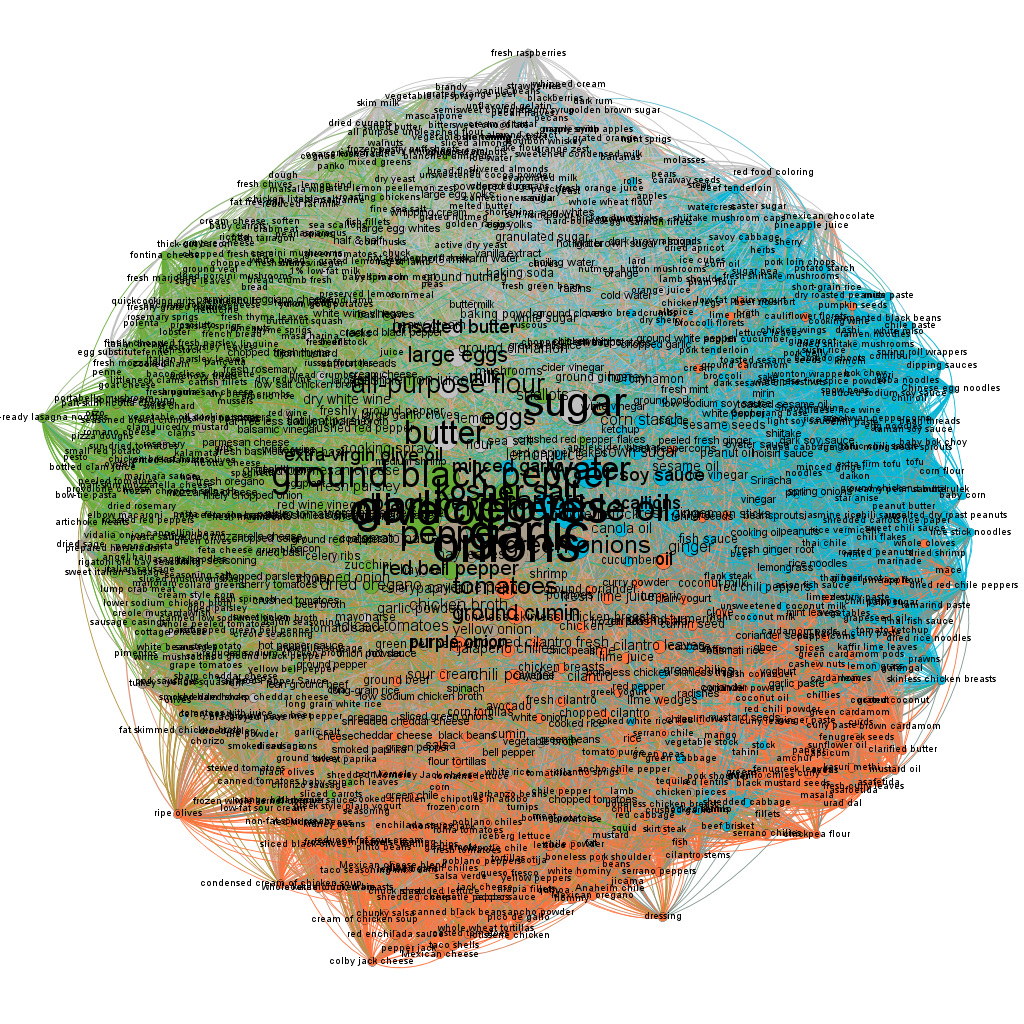
\includegraphics[width=\columnwidth]{images/ingredient_modularity.png}
  \caption{Ingredient Cluster }\label{f:ingredient_modularity}
\end{figure}

Figure \ref{f:ingredient_modularity100} shows ingredient cluster of around 100 nodes. 
\begin{figure}[!ht]
  \centering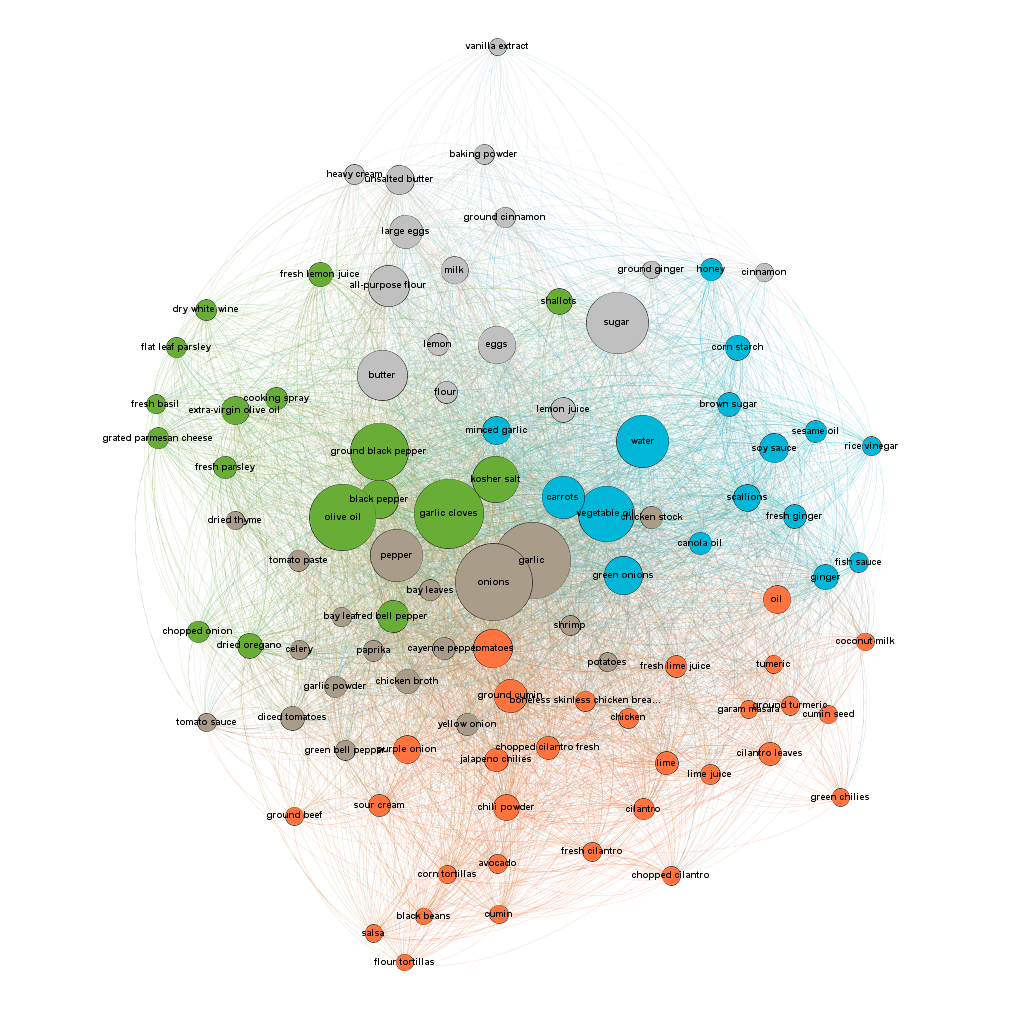
\includegraphics[width=\columnwidth]{images/ingredient_modularity100.png}
  \caption{ingredient Cluster 100 Nodes }\label{f:ingredient_modularity100}
\end{figure}

\subsection{Short Comings/Future Work}



\section{Conclusion}
Hadoop and MongoDB are the front-runner technologies to solve big data problems. The features provided by both technologies are extremely suitable to solve big data problem which requires handling of huge data and great computing power.

\begin{acks}

  The author would like to thank Dr. Gregor von Laszewski for his
  support and suggestions in this project. The author would also like to thanks Kaggle application for hosting ingredient dataset which is used in this project and various online resource which helped in understand and write Python code and Gephi.  

\end{acks}

\bibliographystyle{ACM-Reference-Format}
\bibliography{report} 

\appendix

\input{issues}

\end{document}
